\chapter{Introduction}{
The Web as we know it is mostly a huge collection of documents, e.g. texts,
pictures, \ldots, connected together thanks to HTTP links.
These links carry no meaning about the
relationship between two documents, or about the content a document exhibits.
Linked Data refers to those same documents, but enriched with \emph{semantic}
meta-data. For example, the content of a document can be described by this
meta-data by indicating the language it was written in, or the content's type,
e.g. book or article. Tim Berners-Lee has first introduced the idea of such
enriched web documents, called \emph{Linked Data}. For such a vision to be
viable as the web is now a large collection of heterogeneous data, a framework
that sets the best practices for publishing and searching Linked Data is a
necessity. The \emph{Semantic Web} is such a framework and is not aimed to be a
replacement of the Web as we know it, but as an extension giving relevant
knowledge about documents on the web.
\linebreak

Over the past years, the quantity of Linked Data available has been increasing
and is now reaching a climax. Semantic Data now at hand, the challenge is to be
able to search for information efficiently. Linked Data is commonly stored
within databases called \emph{Triple Stores}, where querying is normally done
thanks to the standardized query language SPARQL defined with the Semantic Web.
However this language, while being very expressive, is known not to scale
efficiently to a large amount of data. \emph{SIREn} is an Information
Retrieval-based search engine which goal is to store and to query efficiently
at the web scale Linked Data. SIREn is a low level application, meant to be
used by other applications such as web services that provide people
information results about what they queried for. \emph{Sindice} is a web
service that provide people and machines a search engine over Linked Data
through the use of SIREn.
\linebreak

SIREn builds an index over the Linked Data collections for searching and
retrieval purpose. With the amount of Linked Data growing quickly, the size of
such indexes and the performance to retrieve data from it are then points of
interest to build a scalable system. A compressed index is of course important
in order to take less space, however decreasing the time spent on IO operations
is also important in order to increase the query throughput. Within the long
studied domain of Information Retrieval, compression methods have been
developed for that purpose. However they were built for traditional indexes,
i.e., indexes built on collections with textual documents (unstructured data). On
the contrary, SIREn builds indexes on Linked Data, i.e., (semi) structured
data. Because the type of data differs, the model used to index documents
is different, which implies that the distribution of indexed values are
different. State of the art compression techniques are not adapted to this new
distribution of values, and so a new compression class has been developed to
match this need: \emph{Adaptive Frame Of Reference}.
\linebreak

Index compression is one aspect that has to be taken care of when building an
efficient and scalable Information Retrieval search engine. Some information
in the index is not relevant to a query. Reading unnecessary data when
processing a query is then wasted time. An other aspect to optimize the
performance of a search engine is to avoid reading useless information with
regards to a query as much as possible by using \emph{self-indexing}
techniques. The \emph{Skip Lists} is a data structure that can be used for that
purpose. Highly efficient compression techniques are nowadays block-based
algorithms. However Skip Lists abstracts from the block view, discarding
statistics about the block that could be used for a more efficient structure.
\emph{SkipBlock} is a block-based self-indexing model that generalizes the
Skip Lists structure.

We review in this report some techniques that aim to reduce the IO access time
overhead in order to increase the overall performance of the Information
Retrieval web search engine. We present AFOR, a compression method that
provides both fast compression and decompression speed, and yet with a high
compression ratio. We propose SkipBlock, a new self-indexing model that
reduces the time of random lookups from inverted lists. }
\section{Motivation}

\subsection{Semantic Web}

\begin{framed}
\begin{quote}
I have a dream for the Web [in which computers] become capable of analyzing
all the data on the Web – the content, links, and transactions between people
and computers. A ``Semantic Web'', which should make this possible, has yet to
emerge, but when it does, the day-to-day mechanisms of trade, bureaucracy and
our daily lives will be handled by machines talking to machines. The
``intelligent agents'' people have touted for ages will finally materialize.
\end{quote}
– Tim Berners-Lee, 1999
\end{framed}

The Semantic Web is an extension of the current Web and acts as a layer of
resource descriptions on top of the current one. These descriptions are
metadata, data about data, that specify various information about web
resources such as their author, their creation date, the kind of the content,
\ldots. Within the Semantic Web framework, \emph{Resource Description
Format}\footnote{\url{http://www.w3.org/TR/2004/REC-rdf-concepts-20040210/\#section-Concepts}}
(RDF) is a standard format that is used to describe a document. RDF adds
information about a web document by embedding metadata. RDF data is structured
data\footnote{Structured data follow a strict a format that allows machine to
understand and process it.}. However semantic data on the Web is large, and each
dataset may have its own schema that may be partially known. They do not all
follow a rigid structure as in databases. We say that the data is
\emph{semi-structured} \cite{abiteboul:1997:icdt}.

Over the past few years, an increasing quantity of Semantic data has been
published on the web, and not just by some programmers but also by industries,
governments and individuals. Some recent RDF data published are:
\begin{itemize}
  \item Governments provide their information to citizens thanks to Linked
  Data such as the British dataset \url{http://data.gov.uk/}, or
  \url{http://data.gov/} by the USA government.
  \item News agents such as the New York Times or Reuters include semantic
  information (i.e., RDF) in their articles.
  \item Web content management systems like Drupal that ease the process to
  expose one's data as structured information for the Semantic Web.
  \item BestBuy\footnote{BestBuy: \url{http://www.bestbuy.com/}} which publishes
  product descriptions, store details and other information in a machine-readable
  format.
\end{itemize}
As per Tim Berners-Lee quote, the semantic web is becoming a reason to get
things moving. The
article\footnote{``The Web Turns 20: Linked Data Gives People Power, Part 1 of
4'' article, which can be found at the address 
\url{http://www.scientificamerican.com/article.cfm?id=berners-lee-linked-data}}
relates some of the possibilities the semantic web gives. It reports that it
allows people to get more involved with the government, e.g. by publishing on
what the public money is being spent on.

\subsubsection{Semantic Web in Action}

A lot of effort has been put in building a set of best practices to make the
Semantic Web viable. This section shall give an overview of this work by first
reviewing prominent ontologies that have been developed to describe knowledge
for a specific domain. Finally we will show an application use case based on Sindice,
called \emph{Sig.ma}, that aggregates Linked Data from different datasets into
one single ``entity profile'', i.e., all resources related to a same entity,
for example such as the entity DERI.

\subsubsection{Publishing Semantic Data}

Tim Berners-Lee, the person credited with coining the terms Semantic Web and
Linked Data, has frequently described Linked Data as ``the Semantic Web done
right''\footnote{slides: \url{http://www.w3.org/2008/Talks/0617-lod-tbl/\#(1)}}.
It aims to create different semantic data datasets of knowledge and to connect
them together. The we can perform a search on a particular dataset, and then to
move to an other dataset because it is somehow related to the current one.
Through a 5-stars Linked Data publishing scheme, Tim Berners-Lee sets the
steps to follow so that individuals and government people contribute in a good
way to enrich the semantic data collection:
\begin{description}
  \item[$\star$] Available on the web (whatever format), but with an open licence
  \item[$\star\star$] Available as machine-readable structured data (e.g. excel
  instead of image scan of a table)
  \item[$\star\star\star$] as (2) plus non-proprietary format (e.g. CSV instead
  of excel)
  \item[$\star\star\star\star$] All the above plus, use open standards from
 W3C\footnote{The World Wide Web Consortium, W3C: \url{http://www.w3.org/}, is
 an international community to build Web standards}, (RDF and SPARQL) to
 identify things, so that people can point at your stuff
  \item[$\star\star\star\star\star$] All the above, plus: Link your data to
  other people’s data to provide context
\end{description}

The Open Data Movement aims at making web data freely available to everyone. The
goal of the Linking Open Data community project is to extend the Web with a
data commons by publishing various open data sets as RDF on the Web and by
setting RDF links between data items from different data sources. RDF links
allow people, and even more so machines, to navigate through the heterogeneous
information. Web data is represented using standard technologies, allowing
data to be reused across applications. The Figure~\ref{fig:LOD} depicts the
current state of the Linking Open Data
Cloud\footnote{\url{http://richard.cyganiak.de/2007/10/lod/}}.

\begin{figure}
\centering
\resizebox{0.8\linewidth}{!}{%
\includegraphics[scale=1]{pics/LOD}
}%
\caption{The Linking Open Data Cloud diagram, where all the current RDF
datasets are presented and how they are interlinked to each other.}
\label{fig:LOD}
\end{figure}

Knowledge can be modeled using a hierarchical structure of relations between the
concepts of a domain, resulting into an \emph{ontology} describing the domain.
Several domains have been represented with ontologies, such as the relations
between people for the social networking, the relations and descriptions of
products for the e-commerce, or even chemistry knowledge in the e-biology. In this
paragraph, some of the developed ontologies are reviewed.

\paragraph{Linked Data for social relations}

\subparagraph{FOAF}

the Friend-Of-A-friend project\footnote{\url{FOAF:
http://www.foaf-project.org/}} is creating a Web of machine-readable pages
describing people, the links between them and the things they create and do,
by using the FOAF ontology. This project create files containing information
about people, who use them in order to describe themselves.
% The Listing~\ref{lst:foaf} depicts a FOAF file, which is 
The FOAF file an HTML document embedding RDF thanks to RDFa\footnote{Resource
Description Framework – in – attributes (RDFa) is a W3C recommendation for
embedding RDF into HTML documents. RDFa:
\url{http://www.w3.org/TR/xhtml-rdfa-primer/}}, created using
\url{http://foaf.me/} and describes my interests, my contact information and
the people I know. By displaying this document into one's homepage, it acts as
an identity profile that can be used by any other applications.

% The lines 2 to 7 inform about the QNames used in the document. For example,
% the family name of the person the FOAF file describes is given by the RDF
% property \emph{foaf:family\_name} in line 15. The lines from 21 to 32 describe
% the people I know and a site that describes them.
% 
% \vspace{1em}
% \begin{lstlisting}[frame=lines, firstnumber=1,
% numbers=left,language=HTML,caption=FOAF file written in the RDF serialization
% format RDFa describing me and the people I know,label=lst:foaf]
% <?xml version="1.0" encoding="ISO-8859-1"?>
% <rdf:RDF xmlns:rdf="http://www.w3.org/1999/02/22-rdf-syntax-ns#"
% 		 xmlns:rdfs="http://www.w3.org/2000/01/rdf-schema#"
%          xmlns:foaf="http://xmlns.com/foaf/0.1/">
% <foaf:PersonalProfileDocument rdf:about="">
%     <foaf:maker rdf:resource="#me"/>
%     <foaf:primaryTopic rdf:resource="#me"/>
% </foaf:PersonalProfileDocument>
% <foaf:Person rdf:ID="me">
%     <foaf:nick>stephane.campinas/scampi</foaf:nick>
%     <foaf:givenname>stephane</foaf:givenname>
%     <foaf:family_name>campinas</foaf:family_name>
%     <foaf:interest rdf:resource="books"/>
%     <foaf:interest rdf:resource="music"/>
%     <foaf:knows>
%         <foaf:Person rdf:ID="friend0">
%             <foaf:name>Giovanni Tummarello</foaf:name>
%             <rdfs:seeAlso rdf:resource="http://g1o.net/"/>
%         </foaf:Person>
%     </foaf:knows>
%     <foaf:knows>
%         <foaf:Person rdf:ID="friend1">
%             <foaf:name>Renaud Delbru</foaf:name>
%             <rdfs:seeAlso rdf:resource="http://renaud.delbru.fr/"/>
%         </foaf:Person>
%     </foaf:knows>
% </foaf:Person>
% </rdf:RDF>
% \end{lstlisting}

\subparagraph{Open Graph Protocol}

In the last few months an increasingly number of web sites have been using
the \emph{``I Like It''}-button provided by FaceBook which tells how many people
like the thing it is attached to. This button also allows to update the
profile of the person who clicked on it. The technology that is actually used is
the \emph{Open Graph Protocol}\footnote{Open
Graph protocol: \url{http://opengraphprotocol.org/}} which is based on the RDF
model. With several RDF property that the protocol defines, a person is able
to give a lot of information. For example, a picture can be further described
by giving it a type (e.g. PNG or GIF), a title or even Geographic locations.
This protocol defines a way thanks to the Semantic Web to represent rich
data, allowing to publish rich information within social sites.

\paragraph{Linked Data for e-commerce}

GoodRelations\footnote{GoodRelations:
\url{http://www.heppnetz.de/projects/goodrelations/}} is an ontology that is
used to describe precisely what a business is offering. Its purpose is to
create a RDF dataset that provides information about products such as its
price, its features or where it is available and so on. Recently, Google
advised\footnote{Google announcement:
\url{http://www.google.com/support/webmasters/bin/answer.py?hl=en&answer=146750}}
merchants to use vocabulary to describe precisely their products, so that they
can be used more efficiently in search results (e.g., related products to the
one searched for, showing in Google search page results). GoodRelations is an
ontology that Google advised to use for this task.

\subsubsection{Semantic Data Mashup}

Sig.ma~\cite{tummarello:2010:sigma} is both a service and an user application
built on top of Sindice that demonstrates the power of the Semantic Web by a
combined use of semantic queries, data aggregation and responsive user
interaction, that together create rich entity descriptions. It can be accessed
online at the address \url{http://sig.ma/}.

\paragraph{Advanced Browsing the Web of Data.}

Starting from a textual search, the user is presented with a rich aggregate of information about the entity likely identified with the query (e.g., a person when the input string is a person name). Queries can be about people, as well as any other entity described on the Web of Data, e.g., locations, name of documents, products, etc. As the user visualises the aggregate information about the entity, links can be followed to visualise information about related entities.

\paragraph{Live views on the Web of Data: rich, embeddable, addressable.}

At any aggregation page, Sig.ma offers rich interactions tools to expand and
refine the information sources that are currently in use as well as some data
oriented cleansing functionalities to hide and reorder values and properties.

As a result, it is possible to interactively create curated ``views'' on the Web
of Data about a given entity which can be then addressed with persistent URLs,
therefore passed in instant messages or emails, or embedded using a specific
markup in external HTML pages. These views are ``Live'' and cannot be spammed:
new data will appear on these views exclusively coming from the sources that
the mashup creator has selected.

\paragraph{Structured property search for multiple entities, Sig.ma APIs.}
A user, but more interestingly an application, can make a request to Sig.ma for
a list of properties and a list of entities. For example requesting ``emails,
affiliation and picture'' for Stephane Campinas, and receiving updated
information about them.

\subsection{Linked Data and Information Retrieval}

With the amount of semantic data growing more each day, a system that is able
to scale and to search efficiently over that data is crucial. Indeed in order
to show the power of the semantic web with applications such as Sig.ma, it is
fundamental that the data structures providing the information are highly
efficient. Information Retrieval techniques have been chosen as a solution.

Information Retrieval deal with the representation and the search of textual
documents. A user express his need for information by issuing a query to the
machine. Information Retrieval systems are nowadays widespread with the daily
use of web search engines by millions of people of Google or Bing to name a
few.

An Information Retrieval search engine is known to scale well
\cite{baeza-yates:2007:icde} to large collections such as the Web. However they
are built for textual documents, i.e., unstructured data, opposed to the
(semi) structured Linked Data. Building an Information Retrieval search engine
for semantic data raises new challenges. Such a search engine has to deal with
highly heterogeneous information sources, to offer advanced search interfaces
and to provide to many simultaneous clients an access to billions of entities
in millions of data sources with sub-second response times. New index
structures as well as new index optimisations are needed to incorporate
semi-structured information in the system while sustaining a fast query
computation and an efficient system maintenance. \emph{SIREn} is a search
engine developed to meet such requirements.	

\section{Internship}

In this section I present how this report is structured, before reporting what
has been achieved during the internship.

\subsection{Outline of this Report}

The report is divided in four parts: the \emph{Background}, the \emph{Methods},
the \emph{Benchmarks} and the \emph{Additional Work and Conclusion}. In the
Background part the different technologies that will be used as a base for the
rest of the document are reviewed. Then in the Methods part I present the
contributions that have been done during the internship. Then the Benchmarks
part reports and discuss evaluation experiments on the new structures
presented in the previous part. Finally some work that has been done on
parallel is reported in the part ``Additional Work and Conclusion''.

\begin{itemize}
  \item[] {\bfseries Part II: Background}\\
In Chapter~\ref{chap:IR} I review the main structures and methods used in
Information Retrieval. In Chapter~\ref{chap:SW} I further describe the RDF data
model representation, since RDF data is the basis of the work done. in
Chapter~\ref{chap:BG-siren} I present SIREn, the search engine for semantic
data using Information Retrieval techniques. In
Chapter~\ref{chap:compression:state-of-the-art} the state of the art compression
techniques are reviewed. The Chapter~\ref{chap:self-indexing} presents a
self-indexing structure, \emph{Skip List}.
  \item[] {\bfseries Part III: Methods}\\
In Chapter~\ref{chap:cmp-methods} I introduce two compression techniques as the
main results of our work. In Chapter~\ref{chap:skipblock} a block-based
self-indexing structure is introduced, based on the Skip List.
  \item[] {\bfseries Part IV: Benchmarks}\\
In Chapter~\ref{chap:benchmarking-framework} the benchmarking framework
throughout the internship in order to perform precise evaluations is described.
In Chapter~\ref{chap:benchmark-cmp} benefits of our new compression technique
are reported, with further experiments on the scalability of the system based
on that compression technique in Chapter~\ref{chap:scalability}. In
Chapter~\ref{chap:self-indexing-bench} the efficiency of the block-based
self-indexing structure is discussed.
\item[] {\bfseries Additional Work and Conclusion}\\
In Chapter~\ref{chap:siren-extension} I present the work that has been done in
parallel on SIREn. In Chapter~\ref{chap:conclusion} I recall what are the main
achievements for this internship and what the future will hold for the author.
\end{itemize}

\subsection{Contribution of the Internship}

During this internship, the work first consisted in develop ping a new high
performance compression technique, \emph{AFOR}, which is more adapted for
compressing data produced by a system like SIREn. Then we worked on developing
a new self-indexing structure, \emph{SkipBlock}, which allows faster document
lookups from the index. A short paper that Renaud Delbru and myself wrote
entitled ``SkipBlock: Self-Indexing for Block-Based Inverted List'', which can
viewed at the Appendix~\ref{app:SkipBlock-paper}, has been accepted for an oral
presentation at the \emph{The $33^{rd}$ European
Conference on Information Retrieval} (ECIR)\footnote{ECIR:
\url{http://www.ecir2011.dcu.ie/}} conference. This conference is an European
forum for the presentation of new research in the field of Information
Retrieval.


\chapter{Digital Enterprise Research Institute} {
DERI is a worldwide organisation of research institutes with the common
objective of integrating semantics into computer science and understanding how
semantics can improve computer engineering in order to develop information
systems collaborating on a global scale. A major step in this project is the
realisation of the Semantic Web.
}
\section{DERI - International}

DERI International is constituted of four research institutes. DERI Innsbruck,
located at the Leopold-Franzens University in Austria, and DERI Galway,
located at the National University of Ireland Galway in Ireland, are the two
founding members and key players. DERI Stanford and DERI Korea are
representative members of DERI in their country and are research institutes
that have joined DERI International. DERI performs academic research and leads
many projects in the Semantic Web and Semantic Web Service field. DERI has been
successfully acquiring large European research projects in the Semantic Web
area such as DIP\footnote{DIP: \url{http://dip.semanticweb.org/}} (Data,
Integration and Processes) or Nepomuk\footnote{Nepomuk:
\url{http://nepomuk.semanticdesktop.org}} (Semantic Web desktop). DERI
collaborates with several large industrial partners as HP, ILOG, IBM and CISCO
but also with medium-sized and small industrial enterprises. DERI is aware of
industry requirements and maintains close relationships with industrial
partners in order to validate research results and transfer them to industry.
DERI also has many research partners, such as the W3C, FZI Karlsruhe or \'Ecole
Polytechnique F\'ed\'erale de Lausanne (EPFL).

\section{DERI - Galway}

DERI Galway was founded in June 2003 by prof.dr. Dieter Fensel and is
currently managed by prof.dr. Stefan Decker. DERI Galway is attached to the
National University of Ireland Galway (NUIG). DERI Galway currently has 130
members composed of senior researchers, PhD students, master and bachelor
students, management staffs and interns. DERI is a Centre for Science and
Engineering Technology (CSET) funded principally by the Science Foundation
Ireland (SFI) but also by Enterprise Ireland, the Information Society
Technologies (EU) and the Irish Research Council for the Humanities and Social
Sciences. DERI divides its research into three main domains
\begin{enumerate}
  \item Social Semantic Information Spaces
  \item Semantic Reality
  \item Application Oriented Research Domain
\end{enumerate}
Within these research strands individual units focus on one core competency
for realising DERI’s mission and its work with its industrial partners. Each
unit specialises in a particular research discipline that has relevance for
realising the overall goals of the institute.

\section{The Mission}

The Web is an area in constant progress, and a major step is on its way:
linking together the real work with the virtual world. A first revolution was
done with the apparition of social networking. This marked an important change
in the way people have been using the Internet: a massive amount of data are
now available and shared. Individuals as well as enterprises gain from it.
However the use of this data is limited because they are platform specific
(e.g. LinkedIn, Facebook, Myspace, \ldots). There are \emph{islands of
information} that do not link to each other.

DERI's mission is to research new technologies that will realise the link
between the real and the virtual worlds (Figure~\ref{fig:deri-mission}): the
development of applications using the semantics of data, software that
inter-connects the islands of information. Two main steps are necessary to
achieve this link:
\begin{enumerate}
  \item \emph{sensors} that collect data from the physical world:
  temperature sensors for home automation, body sensors such as the heartbeats
  to better help people control their health.
  \item \emph{semantic spaces} that break down barriers between information
  allowing their thorough use.
\end{enumerate}
These axes lead to the realisation of linking the real world with the virtual
world, creating what DERI calls the \emph{semantic
reality}~\cite{decker:2008:semantic-reality}.

\begin{figure}
\centering
\resizebox{0.6\linewidth}{!}{%
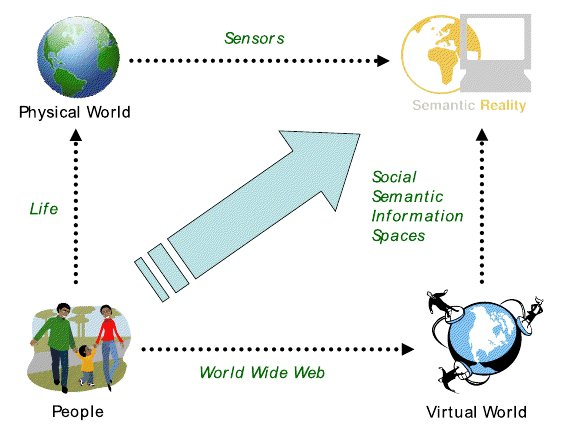
\includegraphics[scale=1]{pics/deri-mission}
}
\caption{Semantic reality.}
\label{fig:deri-mission}
\end{figure}

\subsection{DI2 - Data Intensive Infrastructures}

DI2 position itself within DERI as a unit which purpose is to develop systems
and infrastructures in order to make Social Semantic Spaces a possibility.
The requirements to analyse and understand the inner workings and underlying
fundamental concepts of the Web along with the elevated scalability
requirements for the development of new Web infrastructures have demonstrated
the necessity of Data Intensive Supercomputing (DISC) infrastructures to
support researchers and developers. A prominent characteristic of DISC (as
promoted by major players such as Google, Yahoo and MSN), as opposed to
classic supercomputing, is the importance of very advanced data management
software over high-end hardware configurations. DISC data entries are in fact
known to be formed by hundreds or thousands of commodity machines connected
using common commercial networking infrastructures. It is then up to the
software to be able to deliver high capacity, throughput, scalability,
re-configurability and fault tolerance. To be able to conduct credible
research and development in the Web domain, DERI requires a DISC
infrastructure. As DISC in itself is the subject of ongoing research, the goal
of this work programme is to advance the research and applications of data
intensive infrastructures, to create, maintain and offer to researchers a
state-of-the-art DISC infrastructure, and to research novel algorithms and
data structures for scalable handling of large amounts of semantic
information.

\section{Working Environment}

My internship lasted from February 2010 to December 2010 within the Data
Intensive Infrastructures (DI2) unit. \emph{Sig.ma} is a semantic web
application based on Sindice, the web service that provides search and
retrieval capabilities over semantic data. At the core Sindice uses SIREn, a
search engine based on Information Retrieval, for the purpose of retrieving
semantic data. My supervisors were Renaud Delbru, Ph.D student at the time but
graduated to doctor on December, and Dr. Giovanni Tummarello. The internship
consisted  to assist Renaud Delbru on his thesis about SIREn.

My work was closely watched by my supervisors, with a regular meeting between
R.Delbru and myself in order to discuss the progress, new research ideas,
design and implementations. The research was performed based on other research
scientific publications, in order to provide a solid background for our own
research.

On the hardware aspect, DERI lent me a laptop for the duration of the
internship. Also I had access to DERI servers so that I could perform my own
experiments and benchmarks on a sane environment.

As for the programming languages used during the internship, JAVA and scripting
languages such as shell scripts, ruby, python and sed were used.

